\section{Results}

\subsection{Analog front-end}

The results of the analog front-end (AFE) involves the outputs of the ECG simulator/generator, the preamplifier section and the analog filters, i.e Notch filter and band-pass filter, where the latter is also the output of the AFE.

Initially the figure \ref{fig:afe:1} displays the outputs for each stage in the AFE. It is important to note how the amplitude and its ripples varies by each output. 

\begin{figure}[h!] 
    \centering
    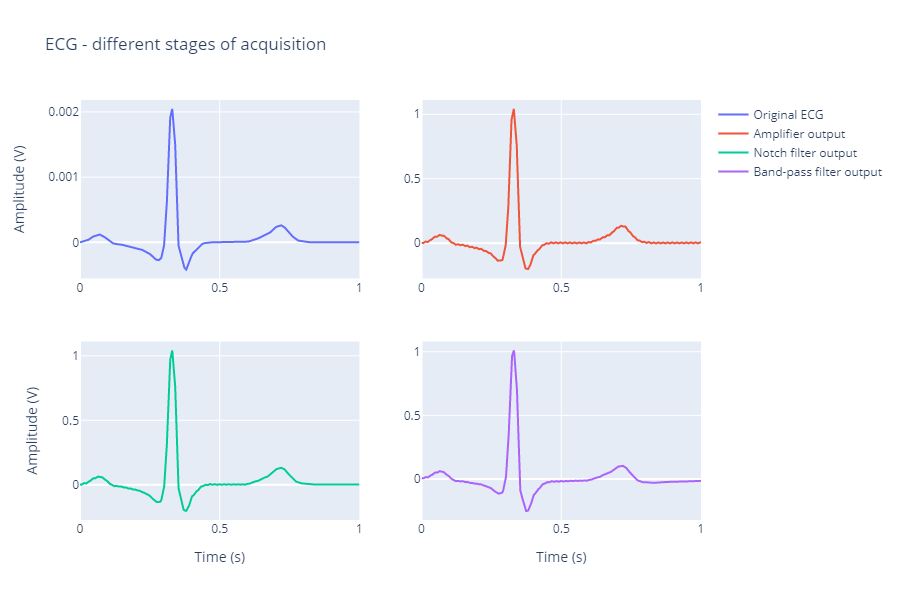
\includegraphics[width=\textwidth]{images/AFE/afe1.png}
    \caption{AFE outputs in time domain from LTSpice.}
    \label{fig:afe:1}
\end{figure}

The ECG simulator generates a low voltage amplitude in mV range, as expected, since the bio potentials measured through the skin follows this behavior. Right after the preamplifier output, the ECG signal reaches an appreciable amplitude, close to a $1 \, V$ peak, but the $60 \, Hz$ ripples remains. Those ripples are attenuated after the Notch filter. At the end, the band-pass filter output does not show great changes in the time domain. A closer look comparing the input and output of the AFE is presented in the figure \ref{fig:afe:2}.

\begin{figure}[h!] 
    \centering
    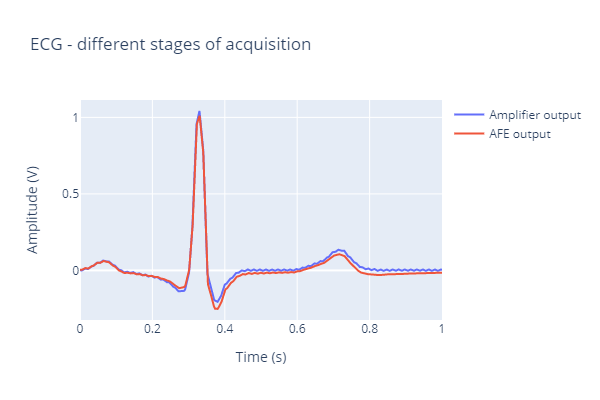
\includegraphics[width=10cm]{images/AFE/afe2.png}
    \caption{Closer look in the AFE outputs in time domain from LTSpice.}
    \label{fig:afe:2}
\end{figure}

Applying the discrete Fourier transform in the LTSpice it can achieve the frequency response of each output, thus revealing more information, like displayed in the figure \ref{fig:afe:4}. 

\begin{figure}[h!] 
    \centering
    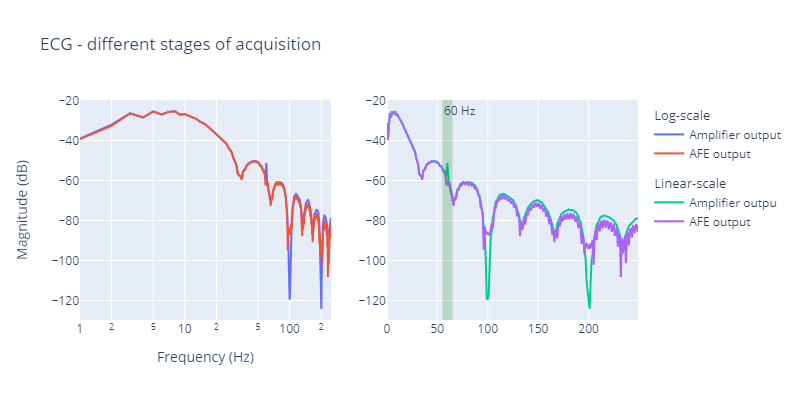
\includegraphics[width=\textwidth]{images/AFE/afe4.png}
    \caption{AFE outputs in frequency domain from LTSpice.}
    \label{fig:afe:4}
\end{figure}

To avoid redundancies in the plots it will only by displayed the amplifier and AFE output (band-pass filter output). This plot shows the direct effect of the Notch filter, reducing the magnitude of the $60 \, Hz$ component. Also is identifiable the band-pass filter result, showing a higher attenuation after the $200 \, Hz$ higher cutoff. Thus ending the AFE analysis.

\subsection{Simulator}

Once the ECG simulator model presented by \textcite{quiroz2019generation} was tested via software and hardware, thus representing two different kinds of plots.

The figure \ref{fig:sim:1} shows a comparison between the ECG generated via software and hardware. The software result was generated via Python, thus allowing the represent float numbers with 32 or 64 bits. Looking for the hardware result that was achieved by the built-in ESP32 8-bit DAC, the quantize output does not show very much precision, indicating the need for a higher resolution DAC or relying in the possibility of transmitting the data via the I2C or I2S protocol with 16-bit resolution to the DAQ. But in general, the hardware output shares reassembles with the original software output.

\begin{figure}[h!] 
    \centering
    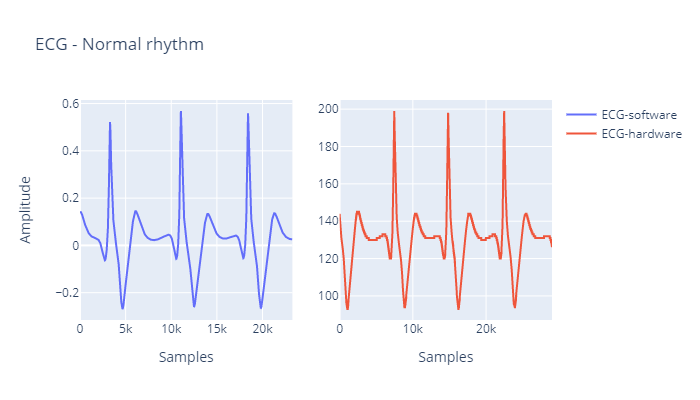
\includegraphics[width=\textwidth]{images/Simulator/simulator1.png}
    \caption{Comparison between ECG generated via software and hardware.}
    \label{fig:sim:1}
\end{figure}

Another characteristic of the ECG simulator is the possibility to generate multiple waveform attached to pre-defined coefficients. With those indicated by \textcite{quiroz2019generation}, it was possibly to generate the pathologies shown in the figure \ref{fig:sim:2}.

\begin{figure}[h!] 
    \centering
    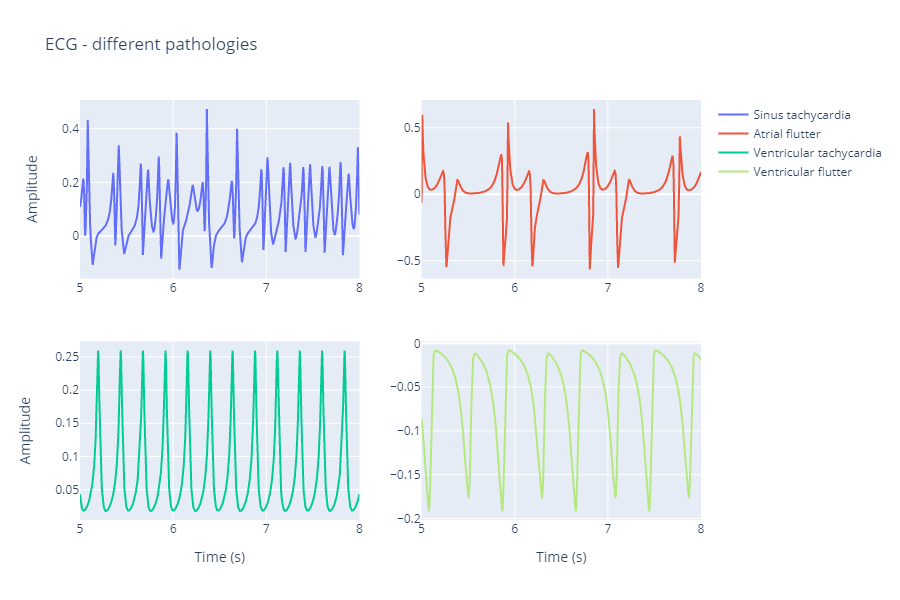
\includegraphics[width=\textwidth]{images/Simulator/simulator2.png}
    \caption{Pathologies simulated.}
    \label{fig:sim:2}
\end{figure}

\subsection{ECG signal processing}

Since the hardware can only store few bytes of data, it is necessary to implement the signal processing algorithms considering the ECG signal windowed. The figure \ref{fig:HR:1} show the high level graphical representation of the windowing, where the window was adjusted bigger than it will be, just for the sake of clean visualization.

\begin{figure}[h!] 
    \centering
    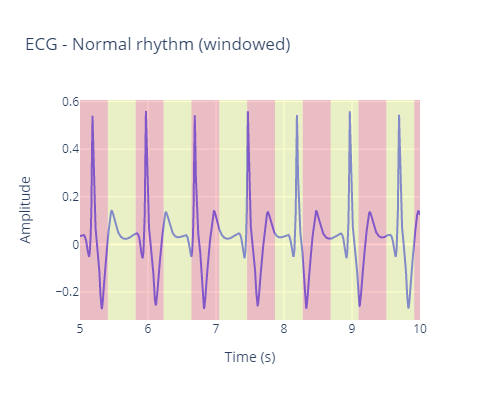
\includegraphics[width=9cm]{images/heart_rate/windowing_software.png}
    \caption{Windowed ECG signal.}
    \label{fig:HR:1}
\end{figure}

\subsubsection{Heart rate}

The heart rate processing generated the figure \ref{fig:HR:2}. The QRS complex peaks that were detected are pointed clearly along the ECG signal and the heart rate evolution is between each peak is presented bellow.

\begin{figure}[h!] 
    \centering
    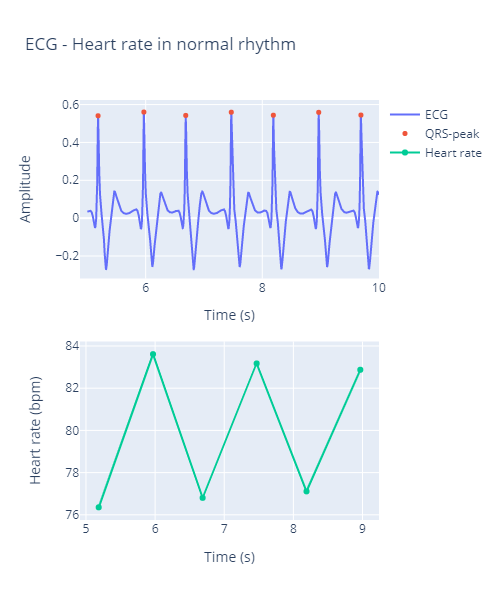
\includegraphics[width=9cm]{images/heart_rate/heart_rate_software.png}
    \caption{Heart rate extracted from ECG signal.}
    \label{fig:HR:2}
\end{figure}

 For the signal of analysis the heart rate remains in the normal rate \cite{clevelandclinic}, once proving that the ECG model truly generates a good approximation for the real signal.

\subsubsection{Pathology analysis}

The pathology analysis is mainly based in the heart rate time-series analysis as shown in figure \ref{fig:HR:3} with heart rate time series for some pathologies addressed in the simulator section. Their detection can be made by just looking to the heart rate time-series, either by tracking any outside normal rate value or checking the high variance in adjacent values of heart rate.

\begin{figure}[h!] 
    \centering
    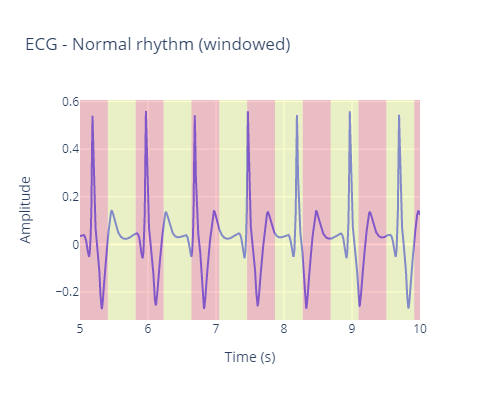
\includegraphics[width=\textwidth]{images/heart_rate/windowing_software.png}
    \caption{Heart rate extracted from ECG signals containing any pathology.}
    \label{fig:HR:3}
\end{figure}
\pagebreak

\subsection{Data acquisition system visualization}

This section address the results regarding the hardware platform of the DAQ that were obtained graphically via the ECG viewer as a Python application in a PC.

The first thing to be analyzed is the moving average filter result in the digital domain. The figure \ref{fig:DAQ:1} shows a noise contaminated ECG signal generated by the ECG simulator and added with a true random number generator noise built in the ESP32.

\begin{figure}[h!] 
    \centering
    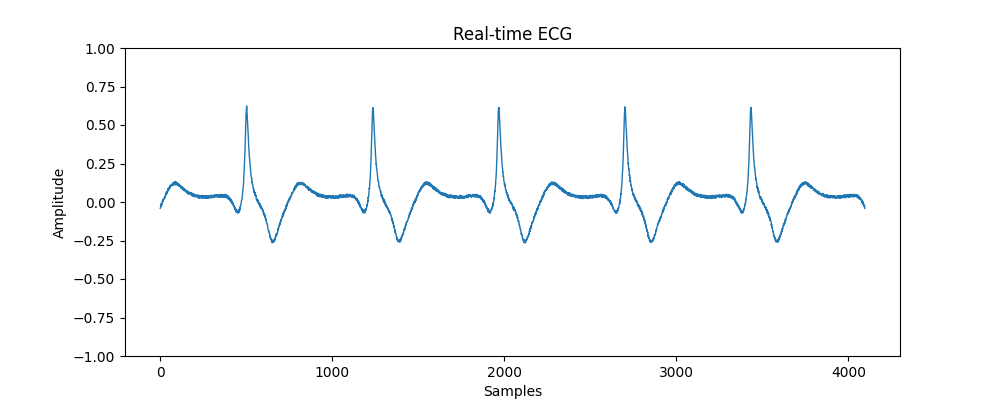
\includegraphics[width=\textwidth]{images/DAQ/daq_ecg_noise.png}
    \caption{ECG viewer displaying a noisy ECG signal.}
    \label{fig:DAQ:1}
\end{figure}
\pagebreak

Right after the noisy ECG passing through the moving average filter explicated in the methodology section, the results become the one in the figure \ref{fig:DAQ:2}. Even using a small kernel of 16 samples, this filter was sufficient to remove major noise problems.

\begin{figure}[h!] 
    \centering
    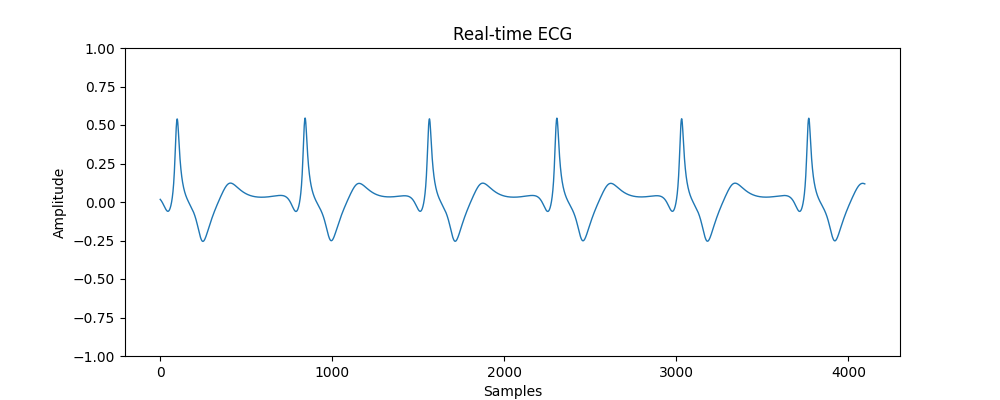
\includegraphics[width=\textwidth]{images/DAQ/daq_ecg_filtered.png}
    \caption{ECG viewer displaying a filtered ECG signal.}
    \label{fig:DAQ:2}
\end{figure}
\pagebreak

Finally the heart rate was also computed in hardware on top of the filtered ECG signal resulting in the figure \ref{fig:DAQ:3} that shows a good interface to monitor the embedded DAQ results.

\begin{figure}[h!] 
    \centering
    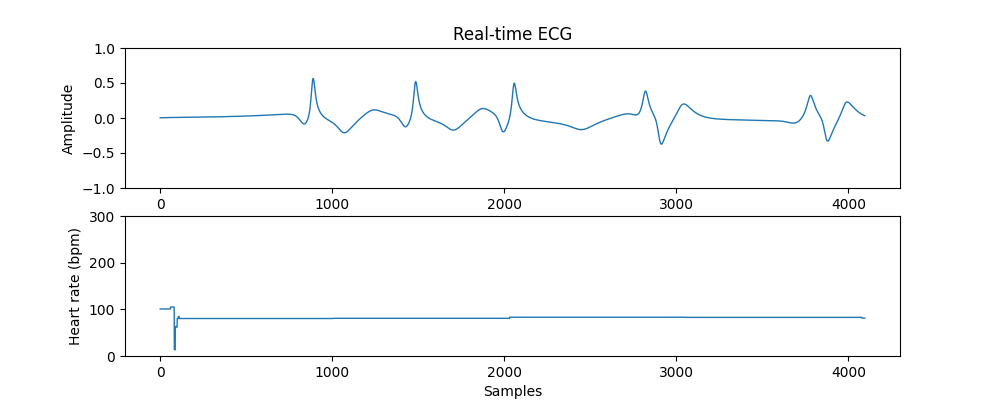
\includegraphics[width=\textwidth]{images/DAQ/daq_heart_rate.png}
    \caption{ECG viewer displaying embedded calculated heart rate.}
    \label{fig:DAQ:3}
\end{figure}
\pagebreak